\documentclass[notes,11pt, aspectratio=169]{beamer}

\usepackage{pgfpages}
% These slides also contain speaker notes. You can print just the slides,
% just the notes, or both, depending on the setting below. Comment out the want
% you want.
\setbeameroption{hide notes} % Only slide
%\setbeameroption{show only notes} % Only notes
%\setbeameroption{show notes on second screen=right} % Both

%\usepackage[scaled=1.0]{helvet}
\usepackage{array}


\usepackage{tikz}
\usepackage{verbatim}
\setbeamertemplate{note page}{\pagecolor{gray!5}\insertnote}
\usetikzlibrary{positioning}
\usetikzlibrary{snakes}
\usetikzlibrary{calc}
\usetikzlibrary{arrows}
\usetikzlibrary{decorations.markings}
\usetikzlibrary{shapes.misc}
\usetikzlibrary{matrix,shapes,arrows,fit,tikzmark}
\usepackage{amsmath}
\usepackage{mathpazo}
\usepackage{hyperref}
\usepackage{lipsum}
\usepackage{multimedia}
\usepackage{graphicx}
\usepackage{multirow}
\usepackage{graphicx}
\usepackage{dcolumn}
\usepackage{bbm}
\newcolumntype{d}[0]{D{.}{.}{5}}

\usepackage{changepage}
\usepackage{appendixnumberbeamer}
\newcommand{\beginbackup}{
   \newcounter{framenumbervorappendix}
   \setcounter{framenumbervorappendix}{\value{framenumber}}
   \setbeamertemplate{footline}
   {
     \leavevmode%
     \hline
     box{%
       \begin{beamercolorbox}[wd=\paperwidth,ht=2.25ex,dp=1ex,right]{footlinecolor}%
%         \insertframenumber  \hspace*{2ex} 
       \end{beamercolorbox}}%
     \vskip0pt%
   }
 }
\newcommand{\backupend}{
   \addtocounter{framenumbervorappendix}{-\value{framenumber}}
   \addtocounter{framenumber}{\value{framenumbervorappendix}} 
}


\usepackage{graphicx}
\usepackage[space]{grffile}
\usepackage{booktabs}

% These are my colors -- there are many like them, but these ones are mine.
\definecolor{blue}{RGB}{0,114,178}
\definecolor{red}{RGB}{213,94,0}
\definecolor{yellow}{RGB}{240,228,66}
\definecolor{green}{RGB}{0,158,115}

\hypersetup{
  colorlinks=false,
  linkbordercolor = {white},
  linkcolor = {blue}
}


%% I use a beige off white for my background
\definecolor{MyBackground}{RGB}{255,253,218}

%% Uncomment this if you want to change the background color to something else
%\setbeamercolor{background canvas}{bg=MyBackground}

%% Change the bg color to adjust your transition slide background color!
\newenvironment{transitionframe}{
  \setbeamercolor{background canvas}{bg=white}
  \begin{frame}}{
    \end{frame}
}

\setbeamercolor{frametitle}{fg=blue}
\setbeamercolor{title}{fg=black}
\setbeamertemplate{footline}[frame number]
\setbeamertemplate{navigation symbols}{} 
\setbeamertemplate{itemize items}[ball]
\setbeamercolor{itemize item}{fg=blue}
\setbeamercolor{itemize subitem}{fg=blue}
\setbeamercolor{enumerate item}{fg=blue}
\setbeamercolor{enumerate subitem}{fg=blue}
\setbeamercolor{button}{bg=MyBackground,fg=blue,}



% If you like road maps, rather than having clutter at the top, have a roadmap show up at the end of each section 
% (and after your introduction)
% Uncomment this is if you want the roadmap!
% \AtBeginSection[]
% {
%    \begin{frame}
%        \frametitle{Roadmap of Talk}
%        \tableofcontents[currentsection]
%    \end{frame}
% }
\setbeamercolor{section in toc}{fg=blue}
\setbeamercolor{subsection in toc}{fg=red}
\setbeamersize{text margin left=1em,text margin right=1em} 

\newenvironment{wideitemize}{\itemize\addtolength{\itemsep}{10pt}}{\enditemize}
\newenvironment{wideenumerate}{\enumerate\addtolength{\itemsep}{10pt}}{\endenumerate}

\usepackage{environ}
\NewEnviron{videoframe}[1]{
  \begin{frame}
    \vspace{-8pt}
    \begin{columns}[onlytextwidth, T] % align columns
      \begin{column}{.58\textwidth}
        \begin{minipage}[t][\textheight][t]
          {\dimexpr\textwidth}
          \vspace{8pt}
          \hspace{4pt} {\Large \sc \textcolor{blue}{#1}}
          \vspace{8pt}
          
          \BODY
        \end{minipage}
      \end{column}%
      \hfill%
      \begin{column}{.42\textwidth}
        \colorbox{green!20}{\begin{minipage}[t][1.2\textheight][t]
            {\dimexpr\textwidth}
            Face goes here
          \end{minipage}}
      \end{column}%
    \end{columns}
  \end{frame}
}

\title[]{\textcolor{blue}{ECN 453: Useful Basic Micro}}
\author[PGP]{}
\institute[FRBNY]{\small{\begin{tabular}{c c c}
Nicholas Vreugdenhil \\
\end{tabular}}}
\date{} 

\begin{document}

% Title Slide
\begin{frame}
\maketitle
  \centering
\end{frame}

% INTRO

\begin{frame}{Plan}
  \begin{wideenumerate}
  	\item Review of demand elasticity
    \item Review of useful terms for this class
  \end{wideenumerate}
\end{frame}

\begin{frame}{Plan}
	\begin{wideenumerate}
		\item \textbf{Review of demand elasticity}
		\item Review of useful terms for this class
	\end{wideenumerate}
\end{frame}

\begin{frame}{Review of demand elasticity}
	  \begin{wideitemize}
	  	\item \textbf{Price elasticity of demand}: Percentage change in quantity demanded for a 1 percent change in price.
	  	\item In math:
	  	\begin{align*}
	  		\epsilon = \frac{dq/q}{dp/p}= \frac{dq}{dp} \frac{p}{q}
	  	\end{align*}
	  \end{wideitemize}
  		\begin{wideitemize}
  			\item Where:
  			\begin{wideitemize}
  				\vspace{11pt}
	  			\item $\frac{dq}{dp}$: slope of the demand curve
	  			\item q: quantity demanded
	  			\item p: price
  			\end{wideitemize}
  		\item \textbf{Notation}: The book sometimes writes demand as e.g. $D(p)=10-2p$ or as e.g. $q=10-2p$. These are equivalent.
  		\end{wideitemize}
\end{frame}

\begin{frame}{Demand elasticity: sign; $\epsilon = \frac{dq}{dp} \frac{p}{q}$ }
\begin{wideitemize}
	\item Since demand slops downwards ($\frac{dq}{dp} \leq 0$) demand elasticity will \textbf{always be (weakly) negative}. 
	\item Economists - confusingly - often just state the magnitude not the sign. 
	\item So, if an economist says `the demand elasticity is 1.2', this does \textbf{not} mean that quantity demanded increases as you increase the price!
	\item Instead, they will be referring to the absolute value (i.e. the true elasticity is -1.2 but the sign is implicit).
\end{wideitemize}
\end{frame}

\begin{frame}{Demand elasticity: example;  $\epsilon = \frac{dq}{dp} \frac{p}{q}$ }
\begin{wideitemize}
	\item \textbf{Question:} 
	\item Demand is given by q = 10 - 3p. Compute the price elasticity of demand at p = 1, q = 7.
	\pause
	\item \textbf{Solution:} 
	\item Compute the slope of the demand curve: $\frac{dq}{dp} = -3$
	\item Plug the slope into the price elasticity of demand formula:
	\begin{align*}
		\epsilon = \frac{dq}{dp} \frac{p}{q} = -3 \times \frac{1}{7} = -3/7
	\end{align*}
\end{wideitemize}
\end{frame}

\begin{frame}{Demand elasticity: classifications $\epsilon = \frac{dq}{dp} \frac{p}{q}$ }
\begin{wideitemize}
	\item $\epsilon < -1$ (e.g. $-1.2$): elastic
	\item $\epsilon = -1$ 
	\item $\epsilon > -1$ (e.g. $-0.8$): inelastic
\end{wideitemize}
\end{frame}

\begin{frame}{Demand elasticity: linear demand; $\epsilon = \frac{dq}{dp} \frac{p}{q}$}
\begin{figure}
	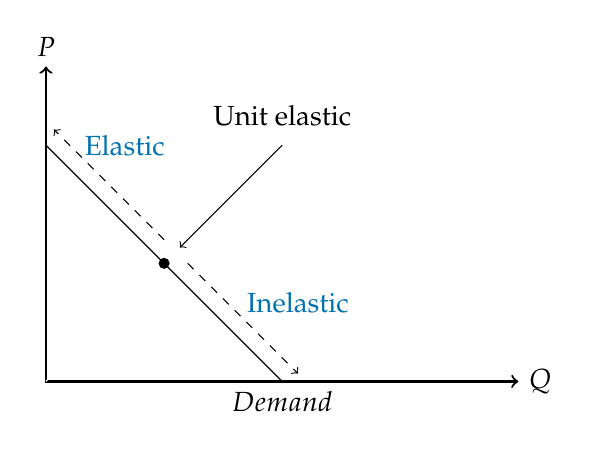
\begin{tikzpicture}[scale=2]
		\draw [<->,thick] (0,2) node (yaxis) [above] {$P$} |- (3,0) node (xaxis) [right] {$Q$};
		\draw [color=white] (0,0) coordinate (a_1) -- (2,2) coordinate (a_2);
		\draw (0,1.5) coordinate (b_1) -- (1.5,0) coordinate (b_2) node [below] {$Demand$};
		\coordinate (c) at (intersection of a_1--a_2 and b_1--b_2);
		\fill [black] (c) circle (1pt);
		\draw[->,dashed] ($(c)+(0,0.15)$) -- ($(c)+(-0.7,0.85)$);
		\draw[->,dashed] ($(c)+(0.15,0.0)$) -- ($(c)+(0.85,-0.7)$);
		\fill [blue] (0.5,1.5) node {Elastic};
		\fill [blue] (1.6,0.5) node {Inelastic};
		\draw[->] (1.5,1.5) node[label= above:Unit elastic] {} -- ($(c)+(.1,.1)$);
	\end{tikzpicture}
\end{figure}
\begin{wideitemize}
	\item \textbf{Note:} Elasticity changes as we move along the demand curve.
	\item Why? Even though the slope $\frac{dq}{dp}$ is constant, the base price and quantity change as we move along the demand curve.
\end{wideitemize}
\end{frame}

\begin{frame}{Demand elasticity: constant elasticity demand curve}
\begin{figure}
	\begin{tikzpicture}[scale=2]
		\draw [<->,thick] (0,2) node (yaxis) [above] {$P$} |- (3,0) node (xaxis) [right] {$Q$};
		\draw [domain=0.5:2.5] plot(\x,1.0 * \x^-1);
	\end{tikzpicture}
\end{figure}
\begin{wideitemize}
	\item Constant elasticity demand curves: $p = a q^{1/\epsilon}$ where $a$ is a number and $\epsilon$ is the the elasticity.
	\item E.g. demand given by $p = 2 q^{1/(-3)}$ has an elasticity of $-3$.
	\begin{wideitemize}
		\vspace{6pt}
		\item (You don't need to know how to prove this, just recognize a constant elasticity demand curve and know how to read off the elasticity.)
	\end{wideitemize}
\end{wideitemize}
\end{frame}

\begin{frame}{Plan}
	\begin{wideenumerate}
		\item Review of demand elasticity
		\item \textbf{Review of useful terms for this class}
	\end{wideenumerate}
\end{frame}

\begin{frame}{Useful terms: revenue}
	\begin{wideitemize}
		\item Total revenue (TR): $TR= p \times q$
		\item Marginal revenue (MR): 
		\begin{wideitemize}
			\vspace{11pt}
			\item Change in total revenue for a 1 unit change in quantity
		\end{wideitemize}
		\begin{align*}
			MR = \frac{d TR}{d q}
		\end{align*}
	\end{wideitemize}
\end{frame}

\begin{frame}{Useful terms: revenue - example}
	\begin{wideitemize}
		\item  \textbf{Example}: Suppose that demand is given by: $p = 4 - 2q$. What is the marginal revenue?
		\pause
		\item \textbf{Solution}:
			\begin{wideitemize}
			\vspace{11pt}
			\item First compute the total revenue:
			\item $TR = p \times q = (4-2q) \times q = 4q - 2q^2$
			\item Next, compute the marginal revenue:
			\item $MR = \frac{d TR}{d q} = 4 - 4q$
			\end{wideitemize}
		\item \textbf{Note:} An important trick is that if demand is \textbf{linear} then marginal revenue has the \underline{same} intercept as demand but \underline{twice} the slope. 
		\begin{wideitemize}
			\item In the above example, demand has a slope of $-2$ and an intercept of 4. Marginal revenue has the same intercept ($4$) but twice the slope ($-4 = 2 \times -2$).
		\end{wideitemize}
	\end{wideitemize}
\end{frame}

\begin{frame}{Useful terms: cost}
		\begin{wideitemize}
			\item Cost function $C(q)$: total cost (TC) of producing $q$ units of output.
			\item Marginal cost (MC): change in TC for a 1 unit change in quantity $q$.
			\begin{align*}
				MC = \frac{d C(q)}{d q}
			\end{align*}
			\item Average cost (AC): the average total cost
			\begin{align*}
				AC = \frac{C(q)}{q}
			\end{align*}
			\item Fixed cost (FC): the total cost at $q=0$ units of output
			\begin{align*}
				FC = C(0)
			\end{align*}
			\item Variable cost (VC): the total cost minus the fixed cost
			\begin{align*}
				VC = TC - FC
			\end{align*}
		\end{wideitemize}
\end{frame}

\begin{frame}{Useful terms: cost - example}
	\begin{wideitemize}
		\item \textbf{Example:} 
		\begin{wideitemize}
			\vspace{11pt}
			\item Suppose that total cost is given by $C(q) = 5 + 10q$. 
			\item What is marginal cost (MC)? What is average cost (AC)? What is fixed cost (FC)? What is variable cost (VC)?
		\end{wideitemize}
		\pause
		\item \textbf{Solution}:
		\begin{wideitemize}
			\vspace{11pt}
			\item $MC = \frac{d C(q)}{d q} = 10$
			\item $AC =  \frac{C(q)}{q} = \frac{5+10q}{q} = 5/q + 10$
			\item $FC = C(0) = 5$
			\item $VC = TC-FC = 5+10q - 5 =10q$
		\end{wideitemize}
	\end{wideitemize}
\end{frame}

\begin{frame}{Useful terms: profits vs producer surplus vs consumer surplus vs total surplus}
	\begin{wideitemize}
		\item Producer surplus (PS) (or `variable profit'): area below the price and above supply curve.
		\item Important:
		\begin{align*}
			\text{total profit = producer surplus - FC}
		\end{align*}
			\item The distinction between profit and producer surplus can often be a little confusing. 
	\begin{wideitemize}
			\item Typically, if fixed costs are not mentioned in a problem then implicitly $FC=0$ and total profit = producer surplus.
	\end{wideitemize}
		\item Consumer surplus (CS): the area above price and below the demand curve.
		\item Total surplus (TS): TS=PS+CS
	\begin{wideitemize}
		\item Note: we use total surplus as a measure of how `efficient' the market is.
	\end{wideitemize}
			\end{wideitemize}
\end{frame}

\begin{frame}{Summary of key points*}
	\vspace{11pt}
	\begin{wideitemize}
		\item Know how to compute the price elasticity of demand from a demand curve and know what is `inelastic' vs `elastic' demand
		\item Know that elasticity changes along a linear demand curve but not along a constant elasticity demand curve
		\item Know what $TR$ and $MR$ mean and how to compute them from a demand curve.
		\item Know the `twice the slope' trick to compute $MR$ from a linear demand curve.
		\item Know what $TC, MC, AC, FC, VC$ mean and how to compute them from a cost function $C(q)$
		\item Know what $PS,CS,TS$ mean and how to compute them.
	\end{wideitemize}
	\vspace{11pt}
	*To clarify, all the material in the slides, problem sets, etc is assessable unless stated otherwise, but I hope this summary might be a useful place to start when studying the material.
\end{frame}

\begin{frame}{References}
	\begin{wideitemize}
		\item Elasticity graph from:
		\item  \url{http://static.latexstudio.net/wp-content/uploads/2016/06/tikzforeconomists-110619150244-phpapp01.pdf}
	\end{wideitemize}
\end{frame}

\end{document}
